\chapter{Progress and Preliminary Results}
\label{ca:chap:progress}

All three hypotheses have now been run once at full scale, with three seeds. This chapter
reports what has been found so far and how confident each finding is. All experiments run
on a shared server with six NVIDIA L40 GPUs (Section~\ref{ca:sec:resources}).

\section{Motivating experiment: the cost of cross-tokenizer supervision}
\label{ca:sec:motivating}

The black-box assumption gives up the teacher's token probabilities. To see what that
costs, on-policy distillation from Qwen3-4B-Instruct was run on Countdown with three
students, each first fine-tuned to the same starting accuracy of about 0.38
(Table~\ref{ca:tab:motivating}). Recovery $R$ is the fraction of the gap between that
starting point and the teacher (0.713) that distillation closed.

\begin{table}[htbp]
\centering
\small
\begin{tabular}{@{}llllc@{}}
\toprule
\textbf{Student} & \textbf{Tokenizer} & \textbf{Loss} & \textbf{Accuracy} & $R$ \\
\midrule
Qwen2.5-1.5B & shared       & exact logits (GKD)                & 0.379 $\to$ 0.600 & 0.66 \\
Qwen2.5-1.5B & shared       & cross-tokenizer loss (ULD)        & 0.379 $\to$ 0.487 & 0.32 \\
OLMo-2-1B    & different    & cross-tokenizer loss (ULD)        & 0.381 $\to$ 0.426 & 0.14 \\
OLMo-2-1B    & different    & GOLD hybrid                       & 0.381 $\to$ 0.035 & collapsed \\
SmolLM2-1.7B & different    & GOLD hybrid                       & 0.375 $\to$ 0.000 & collapsed \\
\bottomrule
\end{tabular}
\caption{On-policy distillation on Countdown with and without a shared tokenizer
(200 steps, 1,000 test puzzles). The first OLMo-2 GOLD run was stopped at step 110.}
\label{ca:tab:motivating}
\end{table}

The cross-tokenizer loss alone halved recovery on a shared tokenizer (0.66 to 0.32; paired
difference $+0.113$, 95\% interval $[+0.091, +0.136]$), and a real tokenizer mismatch
halved it again (0.14). The GOLD hybrid loss, the current method for cross-tokenizer
on-policy distillation, collapsed on both cross-tokenizer students. Its loss kept falling
while accuracy went to zero: it forced OLMo-2 into the teacher's single-digit number
segmentation, which broke its arithmetic, and it let SmolLM2 emit newlines to the length
limit. Logit-level supervision across model families is therefore both lossy and fragile,
which supports building the project on a text-only reward.

\section{Pilot run and what it changed}
\label{ca:sec:pilot}

Every condition was first run once (seed 0, 14.4 GPU-hours) to test the pipeline. Three
findings changed the design. First, the student learned almost only on Countdown, from
0.218 to as much as 0.714 test accuracy; no condition moved MATH or code by more than
0.042, about 1.3 standard errors. A five-times-higher learning rate did not help MATH or
code and cut the Countdown gain from $+0.280$ to $+0.098$, so the rate was kept. Second,
the original headroom selector made the predicted switch from Qwen2.5-3B to Qwen2.5-7B on
Countdown, but then spent 320 of its 400 rounds on MATH, where the headroom never shrank
because nothing was learned. It had no feedback from realised gains, which the revised
selector adds. Third, the original Thompson sampling spent 55\% of its budget on the
degraded provider: dividing noisy gains by cost shrinks the noise of expensive arms towards
zero and so favours them. The revised version estimates gain per round and applies the
price only when choosing. In a simulator calibrated to the pilot, both revised selectors no
longer showed these failures.

\section{Main runs: does adaptivity pay? (H3)}
\label{ca:sec:h3}

Ten conditions were run with three seeds each at $B = 2{,}400$, and every final student was
evaluated greedily on the 1,500 test problems (Table~\ref{ca:tab:h3}).

\begin{table}[htbp]
\centering
\footnotesize
\setlength{\tabcolsep}{2.5pt}
\begin{tabular}{@{}lrccccc@{}}
\toprule
 & & \multicolumn{3}{c}{\textbf{Test accuracy}} & & \\
\cmidrule(l){3-5}
\textbf{Condition} & \textbf{Rounds} & \textbf{Countdown} & \textbf{MATH} & \textbf{Code} & \textbf{Utility [95\% CI]} & \textbf{Diff. [95\% CI]} \\
\midrule
Untrained student & -- & 0.218 & 0.434 & 0.336 & 0.329 & \\
\midrule
Qwen2.5-3B only & 400 & 0.555 & 0.418 & 0.352 & 0.442 [0.416, 0.468] & $-$0.052 [$-$0.083, $-$0.024] \\
Phi-4-mini only & 400 & 0.630 & 0.438 & 0.352 & 0.473 [0.440, 0.508] & $-$0.020 [$-$0.049, +0.009] \\
Qwen2.5-7B only & 364 & 0.698 & 0.423 & 0.360 & 0.494 [0.468, 0.519] & -- \\
Qwen-Coder-7B only & 360 & 0.656 & 0.421 & 0.358 & 0.478 [0.450, 0.507] & $-$0.015 [$-$0.032, +0.000] \\
Phi-4 only & 110 & 0.417 & 0.429 & 0.335 & 0.394 [0.370, 0.417] & $-$0.100 [$-$0.127, $-$0.073] \\
\midrule
Uniform & 223 & 0.556 & 0.437 & 0.343 & 0.445 [0.420, 0.471] & $-$0.048 [$-$0.068, $-$0.026] \\
Headroom, learned eff. & 368 & 0.711 & 0.435 & 0.355 & 0.500 [0.478, 0.523] & +0.007 [$-$0.011, +0.026] \\
Cost-aware Thompson & 400 & 0.508 & 0.435 & 0.346 & 0.430 [0.329, 0.505] & $-$0.064 [$-$0.165, +0.004] \\
\midrule
Correctness, no provider & 200 & 0.611 & 0.425 & 0.352 & 0.462 [0.437, 0.489] & $-$0.031 [$-$0.052, $-$0.011] \\
SFT on responses & -- & 0.373 & 0.421 & 0.322 & 0.372 [0.350, 0.393] & $-$0.122 [$-$0.144, $-$0.099] \\
\bottomrule
\end{tabular}
\caption{Test results of the main runs at budget $B = 2{,}400$, means over three seeds. Utility is the mean of the three domain accuracies. Intervals are 95\% bootstrap intervals over seeds and test items; the last column is the paired difference from the best single provider, Qwen2.5-7B. Rounds are gradient steps, capped at 400; SFT takes no rounds. Runs that reached the cap stopped before spending the whole budget; mean spend was lowest for Qwen2.5-3B alone (1,374 units).}
\label{ca:tab:h3}
\end{table}


\paragraph{The proposed selector matches the best single provider but does not beat it.}
The best single provider is Qwen2.5-7B, with test utility 0.494. The headroom selector with
learned efficiency reaches 0.500, the highest of any condition and the most consistent
across seeds (0.503, 0.498 and 0.500), but its paired advantage of $+0.007$ has a 95\%
interval from $-0.011$ to $+0.026$. H3 is therefore not supported at this budget. The
selector did learn what the pilot version could not: it spent 38 to 58\% of its budget on
Countdown, where learning happens, and only 6 to 9\% on Phi-4. It did not reliably avoid the
degraded provider, which received 16 to 17\% of the budget in two seeds and none in the third.

\paragraph{Other conditions.} Cost-aware Thompson sampling reached 0.465 and 0.502 in two
seeds but collapsed in the third (0.322), where the student's Countdown answers shrank from
445 tokens to 38. Uniform allocation spent 59 to 66\% of its budget on Phi-4 and its degraded
copy and did no better than the cheapest single provider (0.445 against 0.442 for
Qwen2.5-3B). Phi-4 alone was the worst single provider,
because its price bought only 110 rounds. The correctness control, which uses ground-truth
labels and no provider for 200 rounds, reached 0.462, and SFT on provider responses was the
weakest condition at 0.372, below every on-policy run. As in the pilot, all of the gains are
on Countdown: no condition moved MATH or code test accuracy by more than 0.024 from the
untrained student.

These comparisons take the best static allocation over the single-provider runs only. The
planned per-domain allocation, which gives each domain its best provider, is not yet built
(Section~\ref{ca:sec:next}).


\section{Marginal value across domains and over training (H1, H2)}
\label{ca:sec:h12}

All 216 branches have completed. Figure~\ref{ca:fig:mv} shows the measured marginal value of
every provider on every domain at the four checkpoints.

\begin{figure}[htbp]
\centering
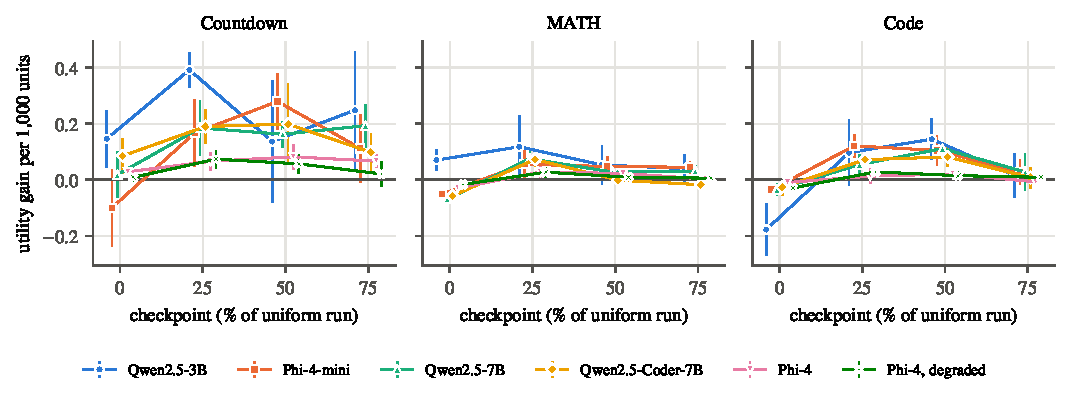
\includegraphics[width=\linewidth]{ca_marginal_value.pdf}
\caption{Marginal value: change in mean selection accuracy over the three domains after
20 rounds on one arm, per 1,000 price units, against the checkpoint the branch started
from. Points are means over three seeds and bars are $\pm 1$ standard error across seeds.
Points are offset horizontally for legibility.}
\label{ca:fig:mv}
\end{figure}

\paragraph{Per unit of budget, cheap providers lead.} On Countdown, the cheapest provider,
Qwen2.5-3B, has the highest mean marginal value at the 0, 25 and 75\% checkpoints, and
Phi-4-mini at 50\%. Qwen2.5-3B is the best Countdown arm in 8 of the 12 combinations of
seed and checkpoint. Per round, without dividing by price, the providers are much closer:
from the 25\% checkpoint, all six raise mean utility by between 0.022 and 0.033 in 20
Countdown rounds. Phi-4 teaches no faster per round, to within noise, than providers that
cost a third as much. It leads only on code from the untrained student, where every
provider lowered utility and Phi-4 lowered it least. The only differences that
are significant in paired comparisons within a seed all involve Phi-4: at 25\%, Qwen2.5-3B
beats Phi-4 and its degraded copy on Countdown, and Phi-4-mini beats Phi-4 on code.

\paragraph{H1 and H2 are not supported at this power.} The decision rules, fixed before the
runs, require the leading provider's 95\% interval to clear its rival's; here these are
t-intervals over the three seeds. With three seeds
this never happens between the cheap and mid-priced providers, at any checkpoint or in any
domain. The leading provider does change between checkpoints and domains, and rankings are
unstable (Kendall's $\tau$ between consecutive checkpoints ranges from $-0.60$ to $0.73$),
but changes of that size are also what noise alone would produce. On MATH and code, every
marginal value is close to zero, consistent with the pilot. The honest summary is that
provider value per unit of budget is dominated by price, that differences among the
affordable providers are smaller than this design can detect, and that H1 and H2 remain
open. Section~\ref{ca:sec:next} plans the measurements needed to settle them.


\section{Issues and limitations found so far}
\label{ca:sec:issues}

\begin{description}[itemsep=2pt,topsep=3pt]
  \item[Learning is concentrated in one domain.] At this scale the student learns almost
    nothing on MATH and code from any provider, or from ground truth. Most of the
    selection problem therefore reduces to how fast each provider teaches Countdown per
    unit of budget. A selector can still win by learning not to spend on MATH and code,
    but H1 and H2 can only be observed where learning happens.
  \item[Statistical power.] Twenty-round branches move selection accuracy by a few points
    at most, and three seeds give wide intervals. The branches also saved only aggregate
    accuracies, so the planned bootstrap over selection-set items cannot yet be computed.
  \item[Training instability.] In the pilot, the student's Countdown responses collapsed
    to a bare answer under Qwen2.5-Coder-7B. This recurred with other providers and in one Thompson
    sampling run, so it is a property of the update, not of one provider, and it is not yet
    understood.
  \item[Simulated providers.] Prices are a compute-based proxy, and providers are open
    models answering from a fixed cache of four responses per prompt. Three of the five
    real providers share the student's model family.
\end{description}
